


\section{Visualisation of clustering}\label{sec:drvis}

In assessing the validity of clustered space, we require a level of exploratory data analysis. To reveal features of interest we plot the reduced 2D dataset and apply interactivity coupled with a selection of visualisation techniques described below. This section outlines the different visualisation methods which have been used.

\subsection{Viewing the 2D species embeddings}
Since the different DR algorithms return data on various scales, comparison between the outputs is not straightforward. To overcome this all outputs in both the $x$ and $y$ directions are normalised (scaled between \{0,1\}), before being plotted as a scatterplot. 


\subsection{Exposing overlapping data}
To be able to interactivity highlight data, a user must first be able to select it. This proved difficult if many of the nodes of a tight-knit cluster are overlapping. As an initial test, node sizes may be reduced, to check if this solves the problem, however, this may often leave points smaller than is possible to easily select. The other solution which was used is to create a force-directed graph where each point is strongly attracted to their initial position. Here we can apply collision detection, whilst still preserving the overall grouping of nodes within a cluster - a technique that was seen in \autoref{ch4}.


\subsection{Gooey Effect (Gaussian Blur)}
Taking a quote from \cite{lessmore}:
\emph{``The more stuff in it, the busier the work of art, the worse it is. More is less. Less is more. %The eye is a menace to clear sight. 
''} and combining it with the work from \autoref{ch1}, we realise that showing each species, when observing overall clusters just add unnecessary clutter to the images. Instead, since we are only interested in the clusters as a unit, a `gooey effect' filter can be applied. This works by merging nearby points into a single water-like blob using a gaussian blur\footnote{Here a gaussian blur of standard deviation 3.7 and a colour matrix [1 0 0 0 0  0 1 0 0 0  0 0 1 0 0  0 0 0 37 -5] is used.}. Here since each point is allocated a colour, if a colour gradient exists, then there are multiple clusters occupying the same place. The aim of this is to reduce the cognitive load on the end-user by reducing the number of distinct objects that they need to take in.



\subsection{Four Colours Theorem}\label{sec:4col}
When plotted, the number of clusters detected often exceeds the number of categorical colours available. In cartography, it has been noted that the colouring of neighbouring polygons should at most take 4 colours. This is the origin of the four colours theorem, \cite{fourcolour}, of which a greedy implementation has been applied.

The aim of this is to show item boundaries (for instance countries, or in our case clusters), whilst reducing ambiguity (if say two neighbours have the same colour). The algorithm I adapted uses the Delaunay tesselation scripts contained within DataDrivenDocuments.js (d3js) \cite{d3js}. This partitions our plane into polygon-regions with boundaries at the furthest distance from each point (Voronoi cells) \cite{delaunay}. First, we chose a random cell and assign it a colour. 
Next, all its neighbours are recursively iterated, giving them the lowest possible colour in a list, which does not match any of their neighbours. Although such a greedy approach does not produce an optimum result it allows for the colouring of data with $\le 5$ distinct colours, as is shown in \autoref{fig:4col}.


\begin{figure}[H]
  \centering
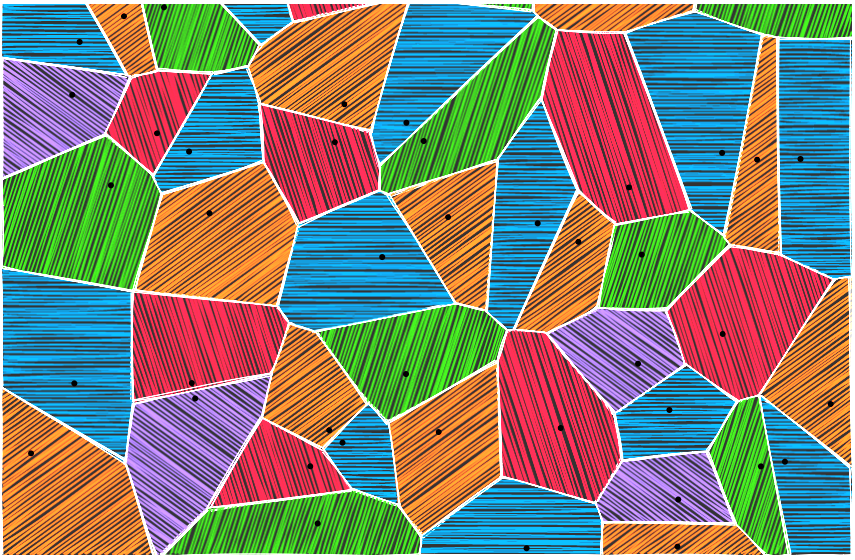
\includegraphics[width=.8\textwidth]{4fig/4col.png}
\caption{\textbf{An example 4 colour matching} This uses the first implementation of the algorithm mentioned in \autoref{sec:4col}. The greedy approach does not often find the optimum solution, which may result in 5 colours instead. Observable Notebook : \cite{4colobs}}\label{fig:4col}
\end{figure}


Having defined all the visualisation techniques we move on to explain the clustering algorithms which are used, and how `goodness of fit' may be measured in the clustering context.

%%%%%%%%%%%%%%%%%%%
%%%%%%%%%%%%%%%%%%%











\section{Cluster Evaluation}
The previous section discussed methods of visualising the reduced data for use with interactive exploratory data analysis. In this section we look at the use of vector clustering algorithms\footnote{Vector clustering is the grouping of data based on their proximity or density to other nearby points} (\autoref{sec:drclustt}) to highlight groups in a 2D dataset, as well an automated method of assessing the quality of the clusters selected (\autoref{sec:silo}) and feature extraction (\autoref{sec:drfeature}).



\subsection{Automated selection of clusters}\label{sec:drclustt}
    When it comes to clustering data points in a dataset, there exist a range of methods which may accomplish a task, \autoref{fig:clustereval}. Most often the k-means, \citep{kmeans}, is used as it is fast and simple to understand. However, its linear method of partitioning cannot capture the splits between non-linear relationships of real data. The other problem is that an estimate for the number of expected clusters is required - something that is often unknown without prior understanding of the data. When this is the case often it is easier to manually select the nodes with interactivity.

In contrast, density-based clustering techniques such as GMM (\citep{scikit}) or DBSCAN (\citep{DBSCAN}) tend to be better at locating non-linear trends in the data. The DBSCAN algorithm asses the distribution of data across a certain location. This allows clusters with a high density of datapoints to be located without the need for a predefined number of clusters. Another method: OPTICS (Ordering Points To Identify the Clustering Structure), \citep{optics}, shall be used\footnote{ If using Python 2, the library for this needs to be extracted from the sci-kit-learn library for python 3 package and altered to run with the previous version. (See copy in attached code.)}. This is an adaptation of the DBSCAN algorithm which does not require the specification of a minimum distance between points (for the density estimate)- instead, we specify a gradient for the distribution and the minimum number of points for a cluster to be classified.


\begin{figure}[H]
     \centering

         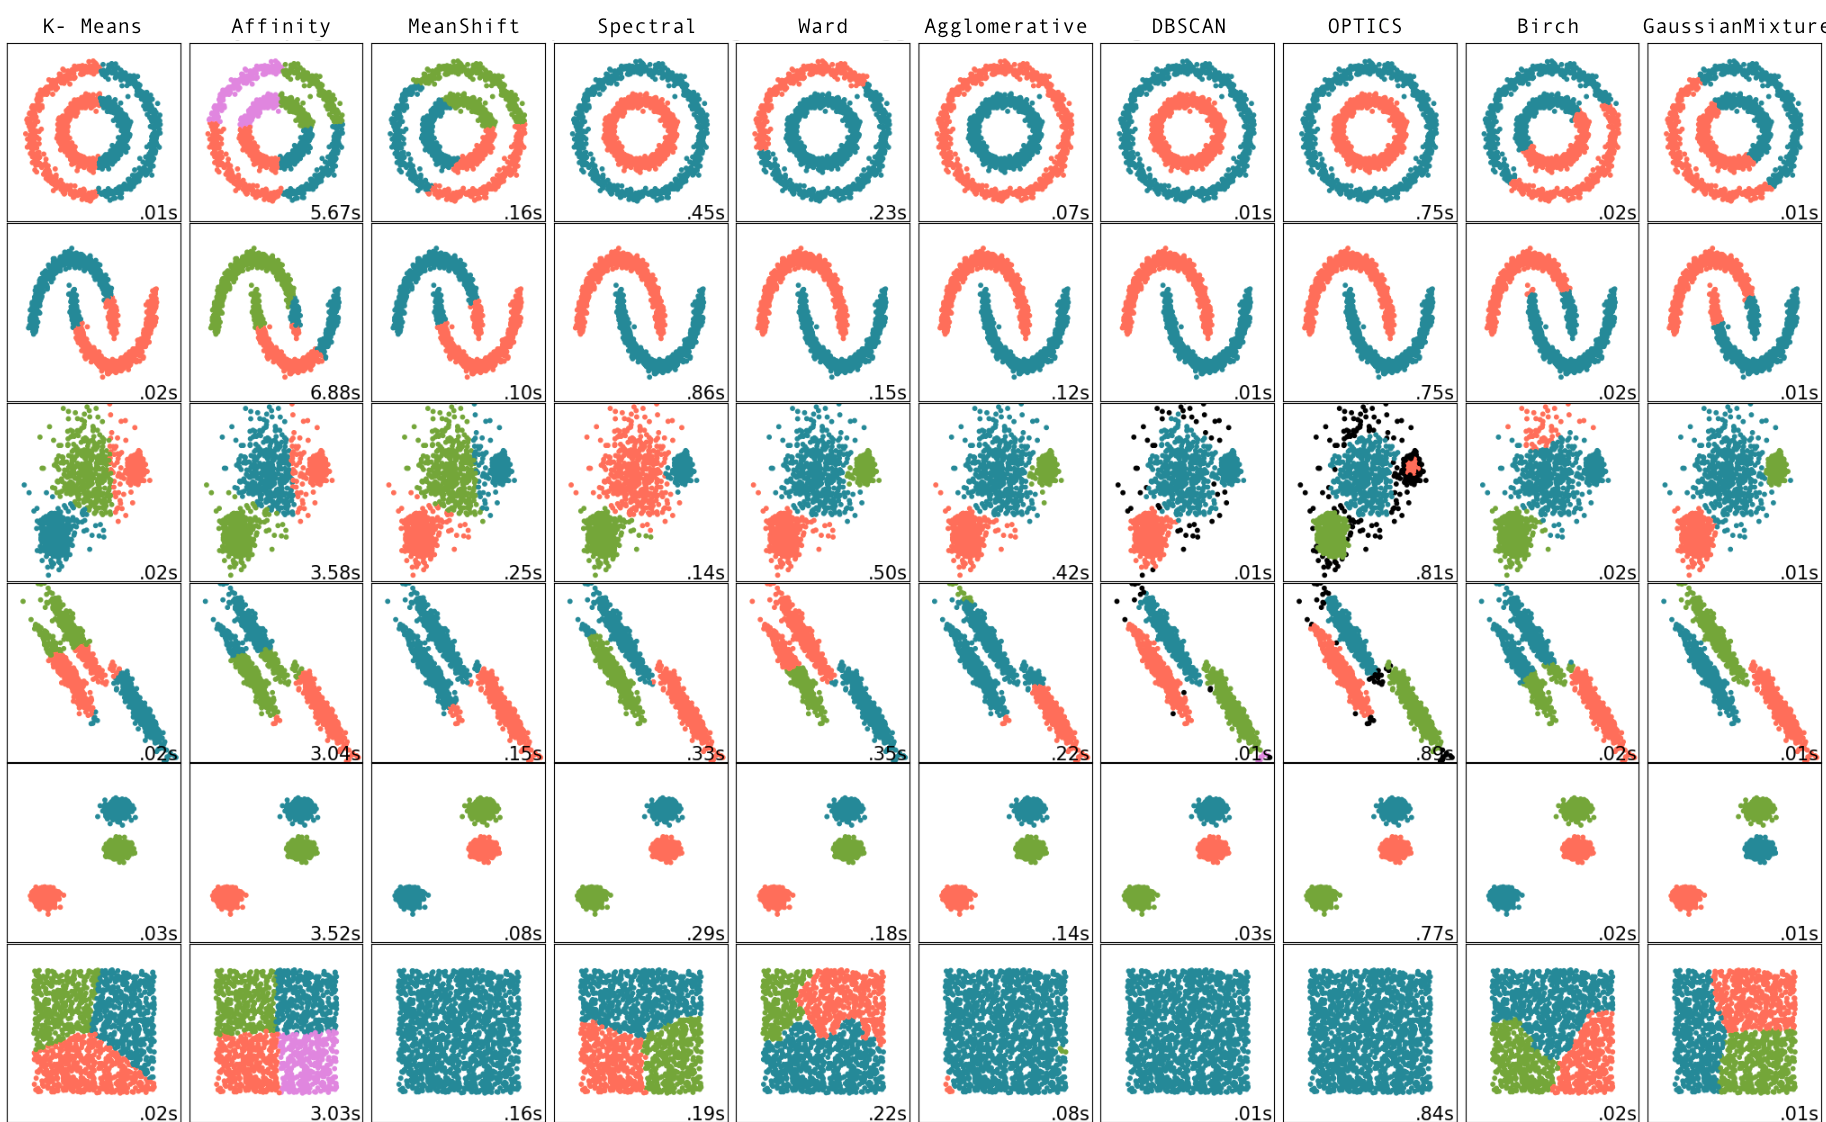
\includegraphics[width=\textwidth]{4fig/clustereval.png}

        \caption{\textbf{A comparison of different clustering methods on a toy dataset.} The plot shows the performance of several vector clustering algorithms in Scikit-Learn. Cluster algorithms are represented across the horizontal axis and several types of datasets are across the vertical. Clustered groups are coloured. Source: \cite{clustereval}}
        \label{fig:clustereval}
\end{figure}


When deciding which algorithms to use, each algorithms' ability to partition non-linear data is considered. 
The first two rows of \autoref{fig:clustereval} show data which cannot be partitioned linearly, here spectral, DBSCAN and optics are the only clustering algorithms to identify both correctly. It is for this reason that we shall look at these for the remainder of the chapter. 

In selecting a value for the results section, several clustering algorithms, with a wide range of input parameters are run. From these, the values with the best silhouette coefficient (\autoref{sec:silo}) are taken. 




\subsubsection{Clustering (Silhouette) coefficient}\label{sec:silo}
The silhouette measure is a tool used for acessing the validity of a set of clusters. Here each cluster is represented as a silhouette, based on the comparison of its tightness and separation. To calculate the silhoette coefficient we look at the intra-cluster $a$ and the mean inter-cluster\footnote{Inside and between different clusters.} distance $b$. The silhouette cluster can then be described using \ref{silhouette,sklearn}:

\begin{equation}
s(i) = \frac{b(i)-a(i)}{\max{ a(i), b(i)}}
\end{equation}

This gives a value $-1 \le s(i) \le 1$. Values near zero suggest overlapping clusters, 1 - dense, well-separated clusters and negative values indicate that a sample may have been incorrectly classified. In using this method we can get an overview of how well individual objects lie within their assigned cluster.




\subsection{Feature Extraction}\label{sec:drfeature}
Upon establishing a set of DR datasets, and their groups (the clusters of species they contain), it is important to evaluate what input features they represent. Rather than doing this manually we make use of Random Forests - described below.

\subsubsection{Random Forrests}
Random forests, \citep{rfrr}, are a subset of ML algorithms called ensemble learning. This means that they train a large number of decision trees, each on a random subset of the original features. A decision tree is a tree formed from a series of conditionals\footnote{Questions with a True/False answer}, much like a perceptron network (\autoref{sec:perceptron}) with binary activation functions. Random forests introduce a level of additional randomness by selecting only a subset on which to create each decision tree. This may introduce a higher bias, but lowers the overall model variance which creates a better (more robust) model. Such methods have been applied to replacing the computationally expensive process of chemistry integration of GEOS-Chem (a global 3D model of tropospheric chemistry) \citep{geosrf} and the prediction of global sea-surface iodine based on observations coupled with sea-surface temperature, depth, and salinity, \citep{iodene}.

\subsubsection{Calculating importance using Random Forrests}
Since random forests are in essence a collection of decision trees, it is possible to generate a `decision tree aggregate' to visualise the ensemble structure of the random forest, \citep{forrester} (\autoref{fig:iodenetree}). Alternatively, if all that is required is the relative importance of each feature, the RandomForrestClassifier from \cite{sklearn} provides a quick and easy way of understanding which features matter, 
\citep{handsonml}. This works by aggregating the weighted nodes which use a certain feature using the number of samples and then scales the result to 1. We use this method to access the overall importance of features within each DR output and identify the differences between clusters.
%bagging an aggregate collection of TreeS


\begin{figure}[H]
     \centering
         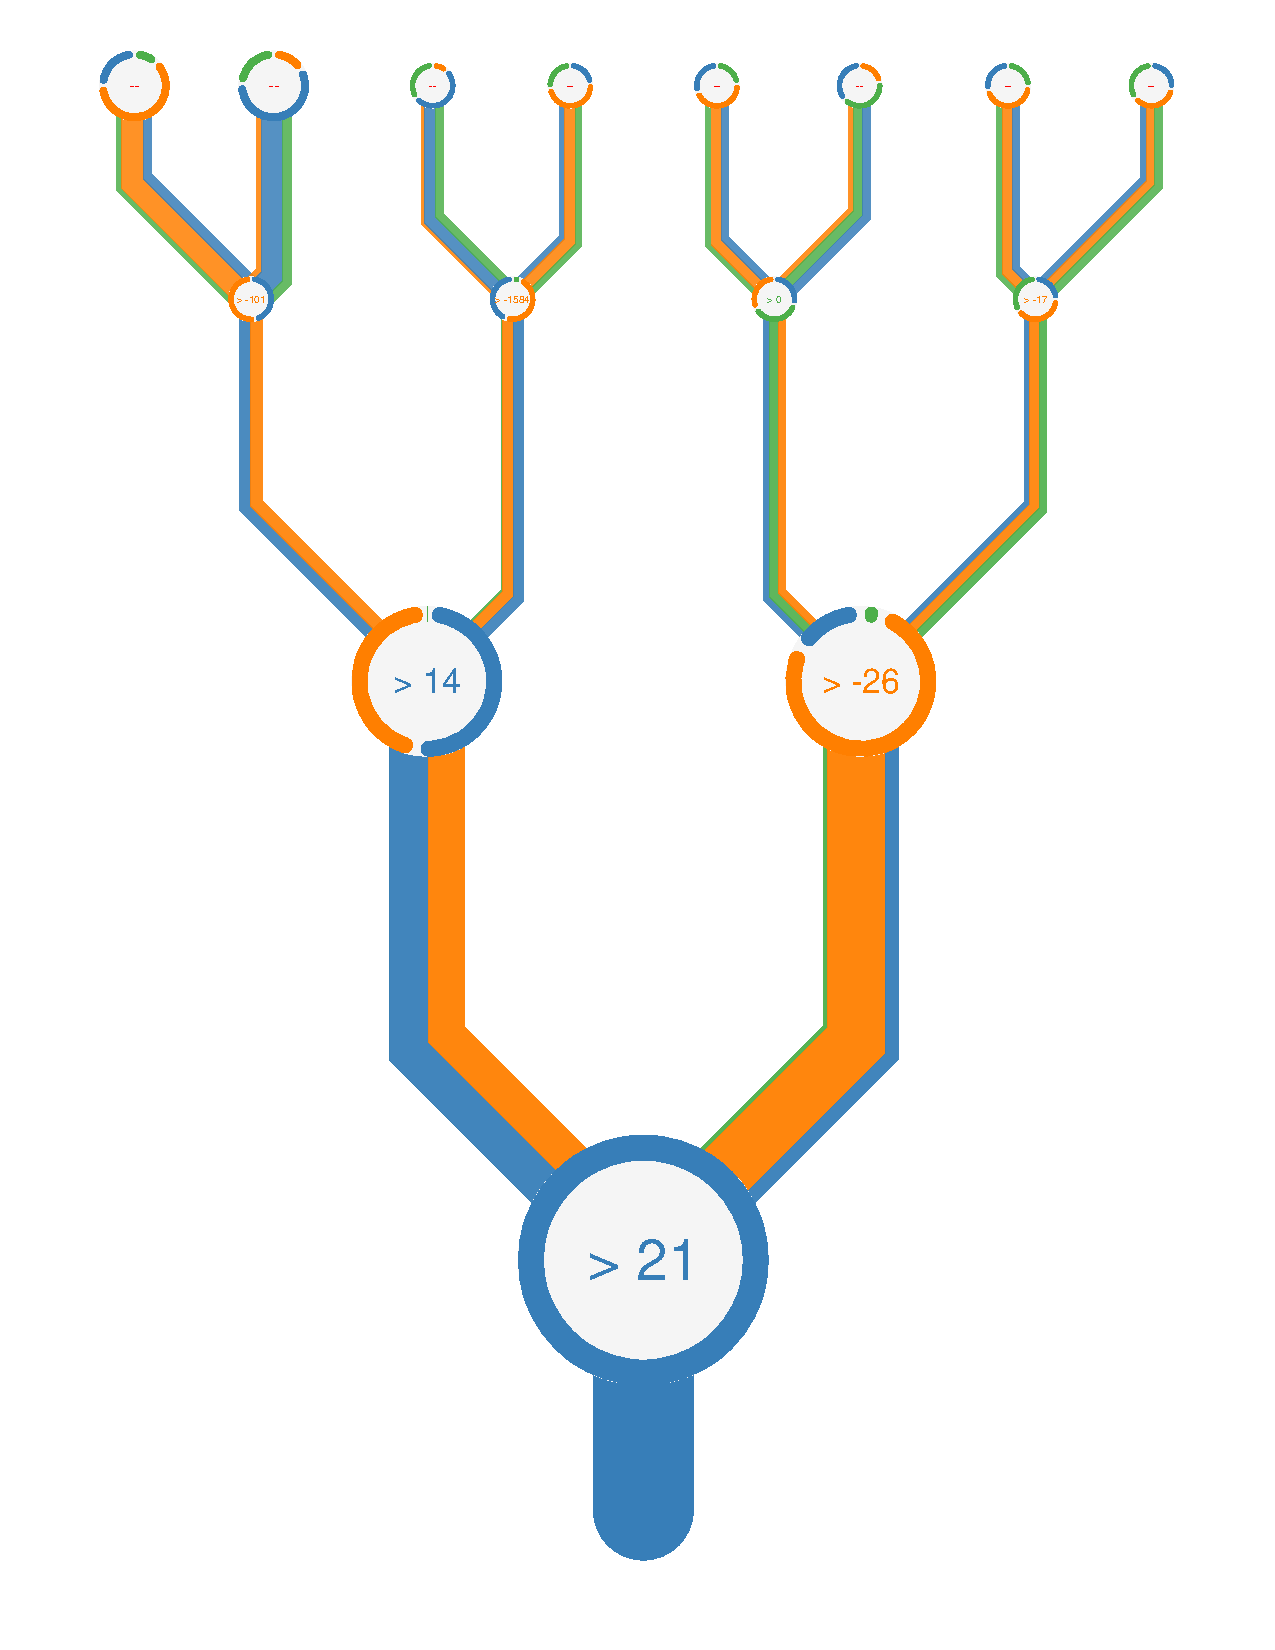
\includegraphics[width=.55\textwidth]{4fig/Oi_prj_features_of_RFR(TEMP+DEPTH+ChlrA)_for_depth_5_white.pdf}
        \caption{\textbf{A decision tree aggrogate from a random forrest plotted with the Epiphyte version of the TreeSurgeon program \citep{forrester}.} The data originates from \cite{iodene} and the imporance of Tempearature (blue), Depth (orange) and Chlorophyll $a$ (green).}
        \label{fig:iodenetree}
\end{figure}


% 
% Random Forrest Classifier from sklearn, top n features.
% https://github.com/MaartenGr/CustomerSegmentation/blob/master/Customer%20Segmentation.ipynb
% https://www.ncbi.nlm.nih.gov/pmc/articles/PMC5732374/

\textit{NOTE: The only downside is that Random Forrests are in themselves ML techniques which also need to be evaluated. To do this, as they are simply being used as indicators of cluster properties which we are to explore further, we can initiate a collection of 300 random Forrest classifiers, from which we take the median. A sort of ensemble learning from an ensemble. }






